\documentclass[11 pt]{article}

\setlength{\oddsidemargin}{-.45in}
%\setlength{\evensidemargin}{-.5in}
\setlength{\textwidth}{7.25in}
\setlength{\topmargin}{-0.95in}
\setlength{\textheight}{10.2in}

\usepackage{graphics}
\usepackage{latexsym}
\usepackage{amsfonts}
\usepackage{amsmath}
\usepackage{amsthm}
\usepackage{epstopdf}
%\usepackage{multicol}
%\usepackage{wrapfig}
\pagestyle{empty}

\usepackage[T1]{fontenc}
\usepackage{baskervald}
\usepackage[bigdelims,vvarbb]{newtxmath} 

\newcommand{\ds}{\ensuremath{\displaystyle}}
\newcommand{\tr}{\vspace{0.5in}}
\newcommand{\lr}{\vspace{1.0in}}
\newcommand{\mr}{\vspace{2.0in}}
\newcommand{\br}{\vspace{3.0in}}

\newcommand{\ps}{Problem Set~}
\newcommand{\vi}{\ensuremath{\mathbf{i}}}
\newcommand{\vj}{\ensuremath{\mathbf{j}}}
\newcommand{\vk}{\ensuremath{\mathbf{k}}}
\newcommand{\vr}{\ensuremath{\mathbf{r}}}
\newcommand{\vecv}{\ensuremath{\mathbf{v}}}
\newcommand{\vu}{\ensuremath{\mathbf{u}}}
\newcommand{\va}{\ensuremath{\mathbf{a}}}
\newcommand{\vs}{\ensuremath{\mathbf{s}}}
\newcommand{\ve}{\ensuremath{\mathbf{e}}}
\newcommand{\vx}{\ensuremath{\mathbf{x}}}
\newcommand{\vc}{\ensuremath{\mathbf{c}}}
\newcommand{\vb}{\ensuremath{\mathbf{b}}}

\usepackage{hyperref} 
\hypersetup{colorlinks=true, linkcolor=blue,  anchorcolor=blue,  
citecolor=blue, filecolor=blue, menucolor=blue, pagecolor=blue,  
urlcolor=blue,pdftitle={MTH 202 Checkpoint}}

\usepackage{framed}

\newcommand{\bdr}{\ensuremath{\mathbb{R}}}

\newcommand{\be}{\begin{enumerate}}
\newcommand{\ee}{\end{enumerate}}

\newcommand{\bi}{\begin{itemize}}  
\newcommand{\ei}{\end{itemize}}

%\renewcommand{\baselinestretch}{1.5}


\begin{document}
 \hfill Boelkins \\
 
\begin{center}
Math 202-06 \\
{\bf Checkpoint 6}
\end{center}


\noindent {\bf Directions:}

\begin{itemize}
	
	\item {\bf Desmos.} You may use \href{https://www.desmos.com/calculator}{\emph{Desmos}} for computations and graphing, just like we do during class.  Any work done in \emph{Desmos} must be summarized and briefly explained in writing on your paper.  
	
	\item {\bf Resources.} During each checkpoint, you may access your own 1 page of study notes, plus \emph{Desmos}; no other uses of your computer or tablet are permitted unless specified directly.  No collaboration with other human beings or other internet resources are allowed.
	
%	\emph{Note well: if you collaborate with someone else, it is often obvious that collaboration has occurred.  Please do not put your academic standing at risk by doing this.}
	
	\item {\bf Competence.} Each week, your goal is to demonstrate competence on as many of the included learning targets as you can.  Each question will be marked either ``Y'' or ``NY'': Y for ``yes'', NY for ``not yet''.  Every learning target will appear on three different checkpoints, so you'll have multiple attempts to demonstrate your understanding.  ``Competence'' is defined as work that demonstrates clear and complete understanding of the relevant concepts in the learning target. While the work may include a minor error, or one or two minor steps may not be well explained, otherwise the work is complete, correct, and convincing, including the proper use of notation, and appropriate explanation of meaning that uses correct terminology.  (On rare occasions, you might get a ``NY*''; such a mark means you are close to competence and that you have the option to have a short conversation with me prior to the next Checkpoint and attempt to demonstrate ``Y''-level understanding through the conversation aloud.)	
\end{itemize}

\noindent \hrulefill \\

\noindent {\bf Learning Targets:} For Checkpoint \#6, there are three learning targets being assessed: 

\begin{quote}
{\bf LT 5}: I can apply an appropriate technique to approximate a definite integral. (Section 5.6)
\end{quote}

\begin{quote}
{\bf LT 6}: I can use definite integrals to find the area between two curves and the volume of a solid of revolution. (Sections 6.1 and 6.2)
\end{quote}

\begin{quote}
{\bf LT 7}: I can use definite integrals to find the mass and center of mass of an object.
\end{quote}

\noindent \hrulefill \\

\vfill \hfill {\bf OVER} 

\pagebreak

\noindent Name: \\ 

\noindent To demonstrate competence on Learning Target \#$n$, you need to correctly respond to all or nearly all of the prompts in question \#$n$.  

\begin{enumerate}

%{\bf LT 5}: I can apply an appropriate technique to approximate a definite integral. (Section 5.6)

\item[5.]  Suppose we know the following information about a function $f(x)$: $f$ is continuous on the interval $[-3,0.6]$, $f$ is either always increasing or always decreasing on the interval, and $f$ is either always concave up or always concave down.  In addition, we have the following data:

	\begin{center}
		\begin{tabular}{l|ccccccccc}
		$x$  &-3.0 & -2.4 & -1.8 & -1.2 & -0.6 & 0.0 & 0.6 \\
		\hline 
		$f(x)$ & 1.6 & 1.7 & 1.9 & 2.3 & 3.05 & 4.0 & 6.2 \\  
		\end{tabular}
	\end{center}

Use the given information to determine the best possible estimate you can for $\ds \int_{-3}^{0.6} f(x) \, dx$. \\  
Start by finding $L_3$, $R_3$, and $M_3$ as estimates of $\ds \int_{-3}^{0.6} f(x) \, dx$, and then use them appropriately to do find the best possible estimate.  \\  

Show a clear summary of your computations using appropriate notation, and write one sentence to explain how you found your final estimate.

\pagebreak

\noindent Name: \\ 

%{\bf LT 6}: I can use definite integrals to find the area between two curves and the volume of a solid of revolution. (Sections 6.1 and 6.2)

\item[6.] For each of the following prompts, {\bf set up, but do not evaluate, a single definite integral that gives the area or volume of each region described}.  Your processes are even more
important than your final answers here, so show all of your work in a clear and logical order. \emph{For each, include a careful, labeled plot, a representative slice, the area/volume of that representative slice, and make
sure your final answer is clearly indicated (for example by circling it).}
	
	
	\be
		\item The exact area of the finite region bounded by the $x$-axis, the curve $x=(2-y)^2-3$, and the line $y = 3-\frac{1}{2}(x+2)$. \\
		
		\scalebox{0.28}{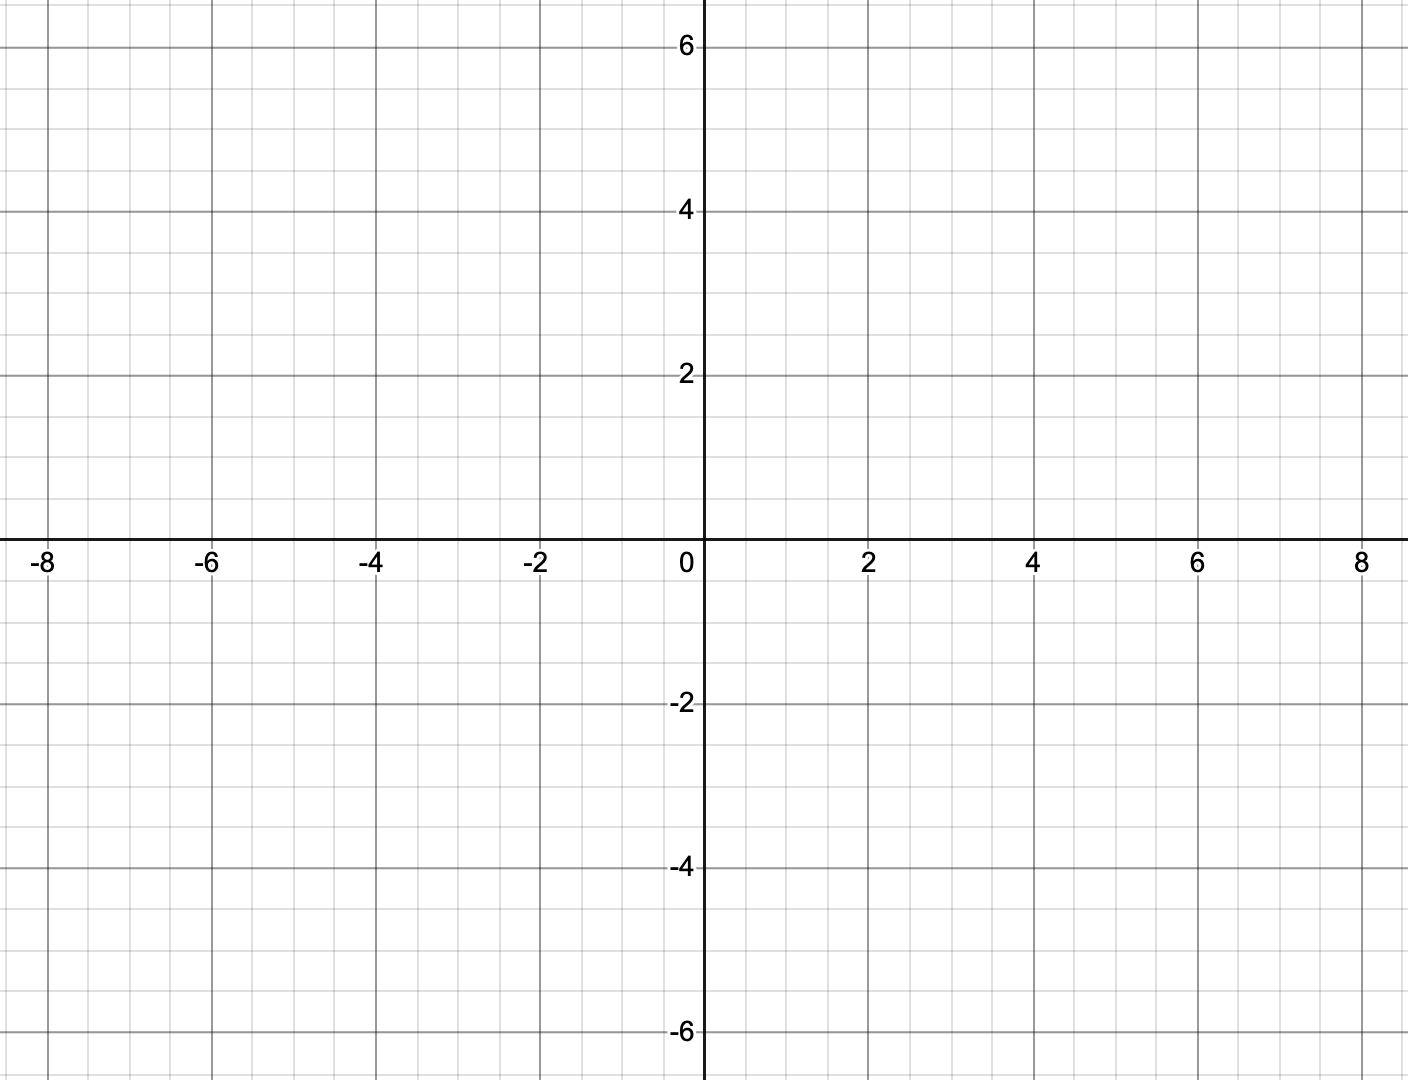
\includegraphics{images/CP-5-blank-grid-LT6.png}} \\
	 	
		\item The exact volume that results from taking the finite region bounded by $x = (y-4)^2$ and $y = 4 - \frac{1}{3}x$ and revolving that region about the $y$-axis. \\
		
		\scalebox{0.28}{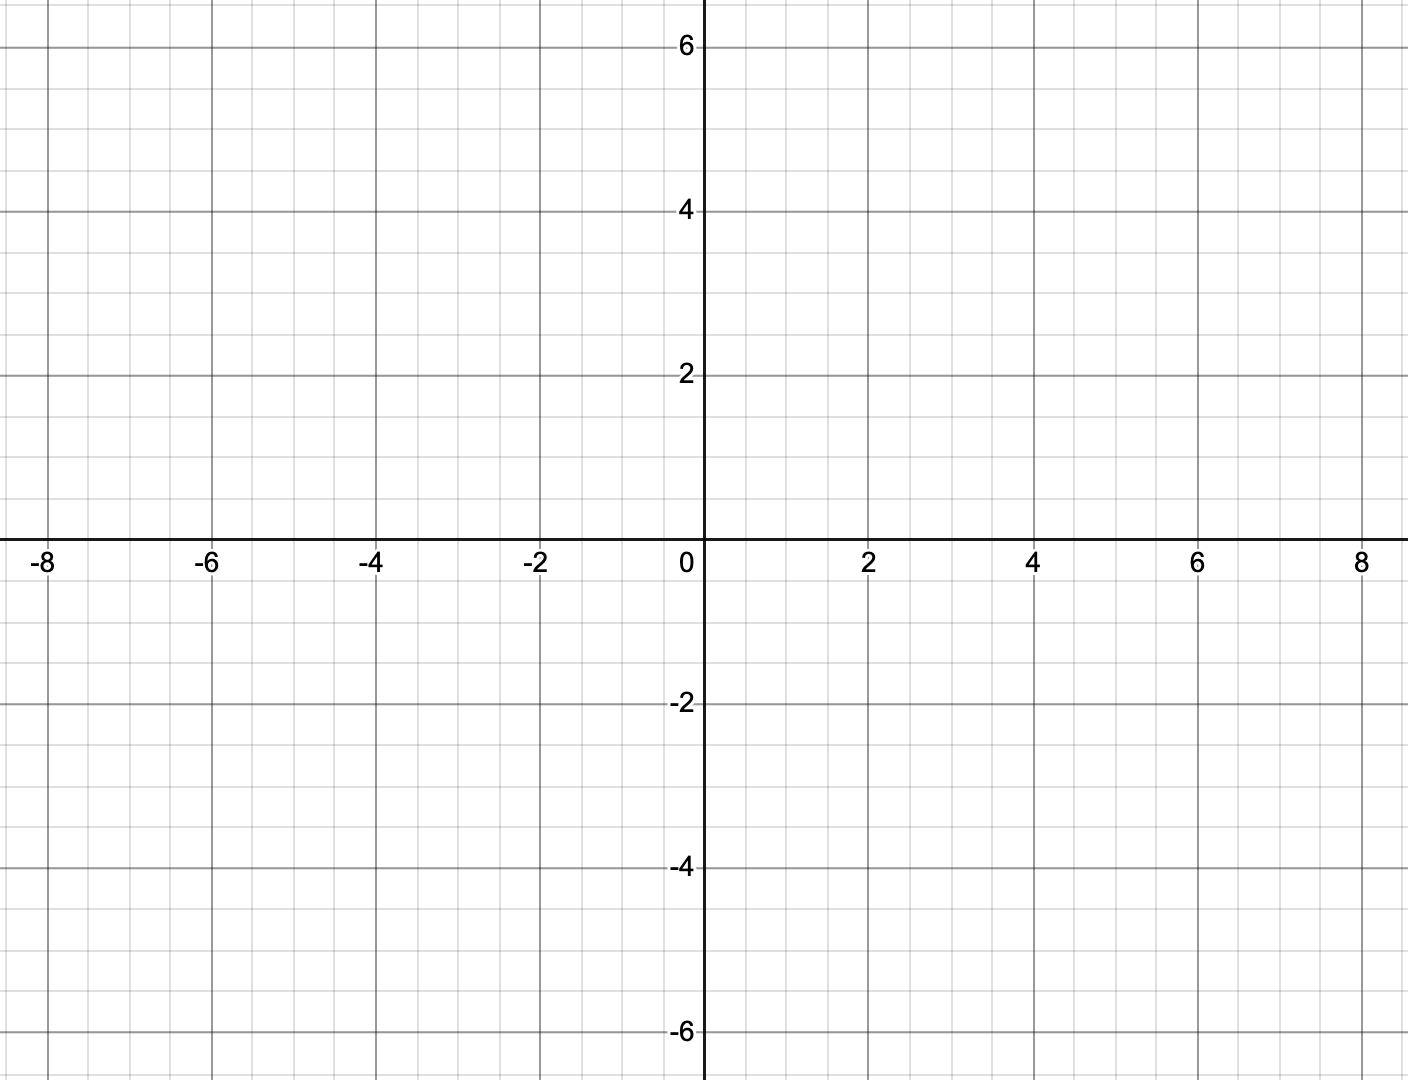
\includegraphics{images/CP-5-blank-grid-LT6.png}} \\
	 	
		\item The exact volume that results from taking the finite region bounded by $x = (y-4)^2$ and $y = 4 - \frac{1}{3}x$ and revolving that region about the $x$-axis.  (This is the same region as in (b).)\\
		
		\scalebox{0.28}{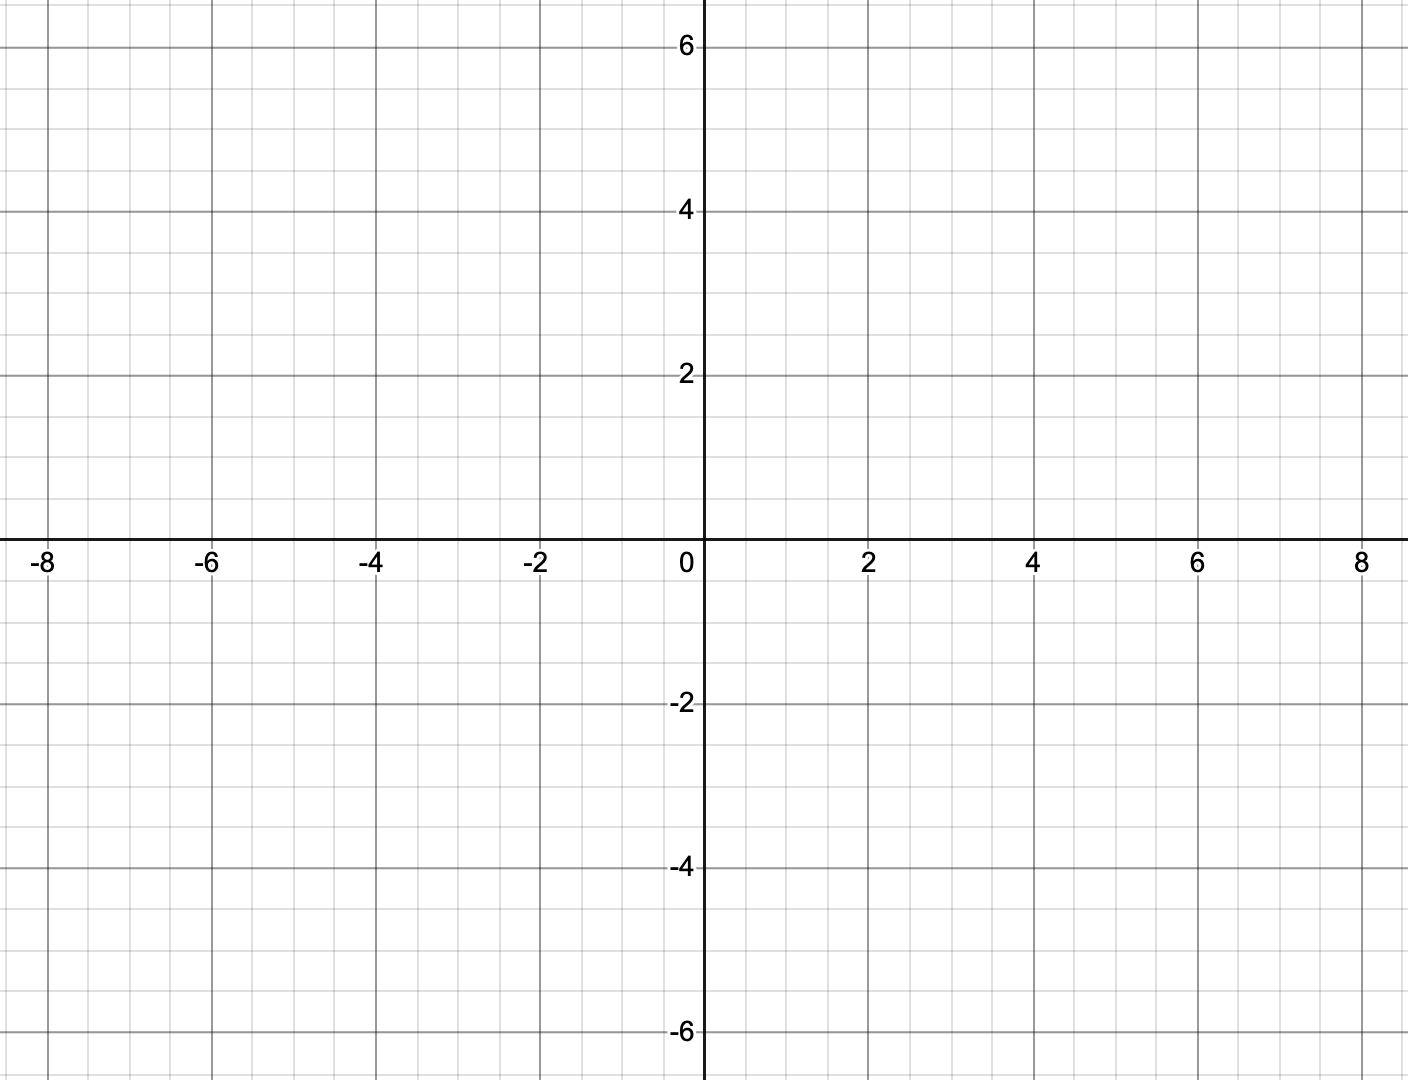
\includegraphics{images/CP-5-blank-grid-LT6.png}} \\		
	\ee


\pagebreak

\noindent Name: \\ 

%{\bf LT 7}: I can use definite integrals to find the mass and center of mass of an object.

\item[7.]  Let a thin rod with constant cross-sectional area of $1$ cm$^2$ be given.  Assume the rod is 2 cm long and is situated so that its left end lies at $x = 0$ on the horizontal axis.  Suppose that the rod's density is distributed along the rod by the function $\rho(x) = 5e^{-x^2}$, measured in grams per cm.

	\be
		\item Without doing any computations, do you expect the rod's center of mass, $\overline{x}$, to lie at $x = 1$, left of $x = 1$, or right of $x = 1$?  Why?
		
		\tr \tr
		
		\item Find the mass $M$ and center of mass $\overline{x}$ by stating appropriate definite integrals and evaluating them using technology.  Clearly identify your results.
		
		\mr \tr
		
		\item Did your work in (b) confirm your intuition in (a)?  Why or why not?  Write a sentence to discuss.
		
		\tr \tr
		
		\item Let $a$ be the value of $x$ for which half of the rod's mass lies to the left of $a$ and half of the rod's mass to the right of $a$.  Will $a$ be equal to $\overline{x}$, lie to the left of $\overline{x}$, or lie to the right of $\overline{x}$?  Why?  Determine the value of $a$ to justify your claim/conclusion.
	\ee	
	
\end{enumerate}



\end{document}
